The purpose of \emph{Object identification} is to assign id's to objects discovered in the current frame based on what was known previous frames and using predictions from the Kalman filter. The aim is to assign a previously detected objects id to the most probable current object, or to none if the previous objects was moving out of the frame. New objects must be given new id's. 

\subsubsection{Error measurement}
Let Object 1 have position and velocity
$$
(x_1, y_1)
$$
$$
(dx_1, dy_1)
$$
The error minimized is then as following below:
$$
  Error_{distance} = (x_1 - x_2 - dx_2)^2 + (y_1 - y_2 - dy_2)^2
$$
$$
  Error_{area} = (|width_1 - width_2| + |height_1 - height_2|)^2
$$
$$
  Error_{total} = Error_{distance} + Error_{area}
$$
If the error is larger than 5000 the error is considered to large and two objects separated by such high error are considered not possibly the same.
\\\\
An error of 5000 equals approximatly
\begin{easylist}
&Approximatly 70 pixels in x- and y-direction apart and having the exact same width/height.
&Approximatly 70 pixels in x- and y-direction apart and having the exact same width/height.
\end{easylist}


\subsubsection{Algorithms}
See code in appendix \ref{sec:ObjID_code}. %referens till kod, ger klickbar länk.

\begin{figure}[htb]
	\centering
	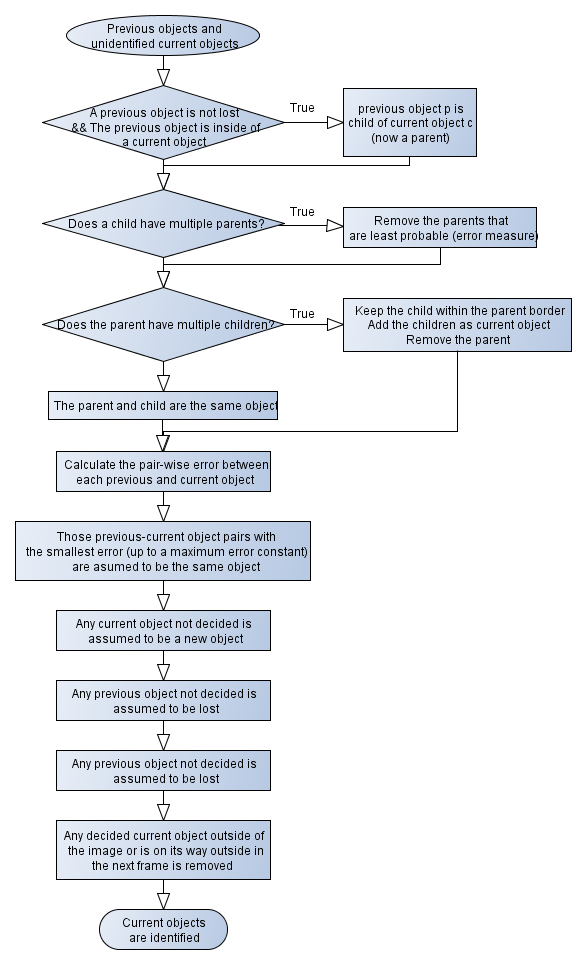
\includegraphics[width=\linewidth]{images/data_flow_identification.png}
	\caption{\textit{Object Identification flowchart.}}
	\label{fig:ObjID_fig} %Skapar referens till figuren
\end{figure}
